\documentclass[11pt,a4paper]{scrartcl}

% ===================== PACKAGES =====================
\usepackage[british,UKenglish,USenglish,english,american]{babel}
\usepackage[tmargin=1in, bmargin=1in, lmargin=0.75in, rmargin=0.75in]{geometry}
\usepackage{tikz}
\usepackage{graphicx}
\usepackage{pgfplots}
\pgfplotsset{width=12cm, compat=1.9}
\usepackage{setspace}
\usepackage{chemmacros}
\usepackage{chemfig}
\usepackage{esint}
\usepackage{tabularray}
\usepackage{makeidx}
\usepackage{epstopdf}
\usepackage{amssymb}
\usepackage{mathrsfs}
\usepackage{bm}
\usepackage{amsmath}
\usepackage{enumitem}
\usepackage[english]{varioref}
\usepackage{lipsum}
\usepackage{fancyhdr}
\usepackage{float}
\usepackage{empheq}
\usepackage[framemethod=tikz]{mdframed}
\numberwithin{equation}{section}
\usepackage{eso-pic}
\usepackage{calc}
\usepackage{nccmath}
\usepackage{caption}
\usepackage{subcaption}
\usepackage{gensymb}
\usepackage{amsfonts, amsthm, epsfig, epstopdf, titling, url, array}
\usepackage{tabularx}
\usepackage{makecell}
\usepackage{booktabs}
\usepackage{array}
\usepackage{siunitx}
\sisetup{input-digits=0123456789\pi}
\usepackage[symbol]{footmisc}
\usepackage{xcolor}
\usepackage{multicol}
\usepackage{boondox-cal}
\usepackage{blindtext}
\usepackage{changepage}

% ===================== SI UNITS =====================
\DeclareSIUnit\atm{atm}

% ===================== PAGE STYLE =====================
\pagestyle{fancy}
\fancypagestyle{firstpage}{\rhead{}}
\fancyhead[L]{\slshape\nouppercase{\leftmark}}
\chead{}
\rhead{}
\lfoot{\textit{}}
\cfoot{-\ \thepage\ -}
\rfoot{\textit{}}
\renewcommand{\headrulewidth}{0.4pt}
\renewcommand{\footrulewidth}{0.4pt}

% ===================== MATH OPERATORS =====================
\DeclareMathOperator{\rank}{rank}
\DeclareMathOperator{\atantwo}{atan2}
\DeclareMathOperator{\spn}{span}

% ===================== COMMANDS =====================
\newcommand{\abs}[1]{\left|#1\right|}
\newcommand{\sign}{\text{sign}}
\newcommand{\centered}[1]{\begin{tabular}{@{}l@{}} #1 \end{tabular}}

% ===================== COLORS =====================
\definecolor{mycolor1}{rgb}{0.97, 0.97, 0.97}
\definecolor{mycolor2}{rgb}{0.97, 0.97, 0.97}
\definecolor{tableShade}{gray}{0.9}

% ===================== THEOREM ENVIRONMENTS =====================
\theoremstyle{it}
\newtheorem{defn}{Definition}[section]
\newtheorem{assumption}{Assumption}[section]
\newtheorem{thm}{Theorem}[section]
\newtheorem{lemma}{Lemma}[section]
\newtheorem{corollary}{Corollary}[section]
\theoremstyle{definition}
\newtheorem{example}{Example}[section]

% ===================== CUSTOM ENVIRONMENTS =====================
\newenvironment{myitemize_1}{
	\begin{itemize}[topsep=0pt]
		\setlength{\topsep}{2pt}
		\setlength{\itemsep}{2pt}
		\setlength{\parskip}{2pt}
		\setlength{\parsep}{2pt}
	}{\end{itemize}}

\newmdenv[
innerlinewidth=0.5pt,
roundcorner=4pt,
backgroundcolor=mycolor2,
linecolor=mycolor1,
innerleftmargin=6pt,
innerrightmargin=6pt,
innertopmargin=6pt,
innerbottommargin=6pt
]{mybox}

% ===================== TABLE COLUMN TYPES =====================
\newcolumntype{Y}{>{\hsize=2\hsize}X}
\newcolumntype{Z}{>{\centering\arraybackslash\hsize=0.857\hsize}X}

% ===================== SECTION DEPTH =====================
\setcounter{secnumdepth}{3}
\setcounter{tocdepth}{3}

\title{\textbf{ 
	\begin{LARGE}
		Power Supply 25V 12kA:
	\end{LARGE} \\[12pt]
	\begin{LARGE}
		technical report.
	\end{LARGE}
	}
}
\author{\textbf{Secom srl, Davide Bagnara}}

\begin{document}
	\thispagestyle{firstpage}
	\begin{mybox}
		\maketitle
		\vspace{100mm}
	\end{mybox}
	\newpage
	\tableofcontents
	\listoffigures	
	\listoftables
	\newpage
	
%\chapter*{}	
%\begin{adjustwidth}{50pt}{50pt}
%		\textit{In the present document the design and model derivation of a CLL-Resonant DC/DC converter is reported. The document includes the control strategy and additional control loops for load harmonic compensation.}
%\end{adjustwidth}
\section*{Nomenclature}
\begin{itemize}
	\item[--] AFE: active front end;
	\item[--] PS-FBC: phase shif full bridge converter;
	\item[--] LCL: inductor-capacitor-inductor filter layout;
	\item[--] $\text{THD}_\text{i}$: current total harmonic distortion;
	\item[--] $L_\text{grid}\quad\Big[\SI{}{\henry}\Big]$: point of common coupling ({PCC}) inductance and \emph{LCL} output filter inductance;
	\item[--] $C_\text{Fu}\quad\Big[\SI{}{\farad}\Big]$: \emph{LCL} output filter capacitor;	
	\item[--] $R_\text{CFu}\quad\Big[\SI{}{\ohm}\Big]$: damping of the LCL output filter capacitor;	
	\item[--] $L_\text{Fu}\quad\Big[\SI{}{\henry}\Big]$: \emph{LCL} input filter inductance;	
	\item[--] $C_\text{Fi}\quad\Big[\SI{}{\farad}\Big]$: dclink capacitor of the AFE stage;	
	\item[--] $C_\text{dc}^{dc1}\quad\Big[\SI{}{\farad}\Big]$: input capacitor of the PS-FBC stage;	
	\item[--] $C_\text{dc}^{dc2}\quad\Big[\SI{}{\farad}\Big]$: output capacitor of the PS-FBC stage;	
	\item[--] $L_\text{dc}^{dc2}\quad\Big[\SI{}{\farad}\Big]$: output inductance of the PS-FBC stage;
	\item[--] $L_\text{s}\quad\Big[\SI{}{\henry}\Big]$: series inductance of the PS-FBC stage;	
	\item[--] $\vec{u}_\text{g}^\text{abc}(t)\quad\Big[\SI{}{\volt}\Big]$: grid voltage used by AFE for PLL grid synchronization;	
	\item[--] $\vec{i}_\text{g}^\text{abc}(t)\quad\Big[\SI{}{\ampere}\Big]$: grid current used PF and THDi evaluation;	
	\item[--] $u_\text{dc}^\text{dc1}(t)\quad\Big[\SI{}{\volt}\Big]$: AFE stage dclink voltage;	
	\item[--] $u_\text{ac}^\text{ac1}(t)\quad\Big[\SI{}{\volt}\Big]$: transformer input voltage;			
	\item[--] $i_\text{ac}^\text{ac1}(t)\quad\Big[\SI{}{\ampere}\Big]$: transformer input current;		
	\item[--] $i_\text{d}^\text{dn}(t)\quad\Big[\SI{}{\ampere}\Big]$: n-th diode rectifier current;	
	\item[--] $f_\text{pwm}^\text{afe}\quad\Big[\SI{}{\hertz}\Big]$: AFE switching frequency;
	\item[--] $f_\text{pwm}^\text{fbc}\quad\Big[\SI{}{\hertz}\Big]$: PS-FBC switching frequency.		
\end{itemize}
\begin{onehalfspace}
\section{Introduction}

The system described in this document is designed to deliver a nominal output voltage of \SI{25}{\volt} at \SI{12}{\kilo\ampere},
corresponding to a rated power of \SI{300}{\kilo\watt}, from a three-phase \SI{480}{\volt} mains supply.

The document is structured as follows. Section~\ref{sec:specs} summarises the electrical
and thermal specifications together with the two operating conditions defined for
compliance verification: nominal load cold (\emph{NLC}) and nominal load hot (\emph{NLH}).
Section~\ref{sec:topology} presents the selected topology and justifies the design choices
with respect to efficiency, current ripple, and controllability.
The converter design — including transformer architecture, switching-stage sizing, and
output filter — is detailed in Section~\ref{sec:design}. Control strategy and
measurement chain accuracy are addressed in Section~\ref{sec:control}, and thermal
management is discussed in Section~\ref{sec:thermal}.

\section{Power Supply Specification}\label{sec:specs}
In this section a list of requirements and constraints which the power supply shall satisfy is reported. 

\begin{itemize}
	\item[--] Overall performance and requirements:
	\begin{itemize}
		\item[--] Nominal Output Voltage, $V_\mathrm{out}^\mathrm{nom} = \SI{25}{\volt}$.
		\item[--] Nominal Output Current, $I_\mathrm{out}^\mathrm{nom} = \SI{12}{\kilo\ampere}$.
		\item[--] Nominal Output Power, $P_\mathrm{out}^\mathrm{nom} = \SI{300}{\kilo\watt}$.
		\item[--] Maximum Output Voltage Ripple, $\Delta v_\mathrm{out} \le \SI{0.25}{\volt}$ (rms).
		\item[--] Current accuracy, $\lvert\tilde{i}\rvert_\mathrm{max} \le \SI{1}{\percent}$.
		\item[--] Voltage accuracy, $\lvert\tilde{v}\rvert_\mathrm{max} \le \SI{0.5}{\percent}$.
		\item[--] Efficiency, $\eta > \SI{90}{\percent}$.
		\item[--] The power supply shall provide galvanic isolation.
		\item[--] Maximum grid current distortion, $\mathrm{THD}_i < \SI{5}{\percent}$.
		\item[--] Power Factor, $\mathrm{PF} > \num{0.95}$ over the entire operating range.
	\end{itemize}
	\item[--] Electrical power source specifications:
	\begin{itemize}
		\item[--] Grid Voltage, $V_\mathrm{grid} = \SI{480}{\volt}$,
		operative range \SI[retain-explicit-plus]{+5}{\percent}~/~\SI{-10}{\percent}.
		\item[--] Grid Frequency, $f_\mathrm{grid} = \SI{50}{\hertz}$ / \SI{60}{\hertz},
		$\pm\SI{2}{\percent}$.
		\item[--] Short-Circuit Current at PCC, $I_\mathrm{cc} = \SI{15}{\kilo\ampere}$.
	\end{itemize}
	\item[--] Liquid cooled (de-ionized water not specified).
	\item[--] Operative working condition as shown in Figure~\ref{current_profile}.
\end{itemize}

\begin{figure}[H]
	\centering
	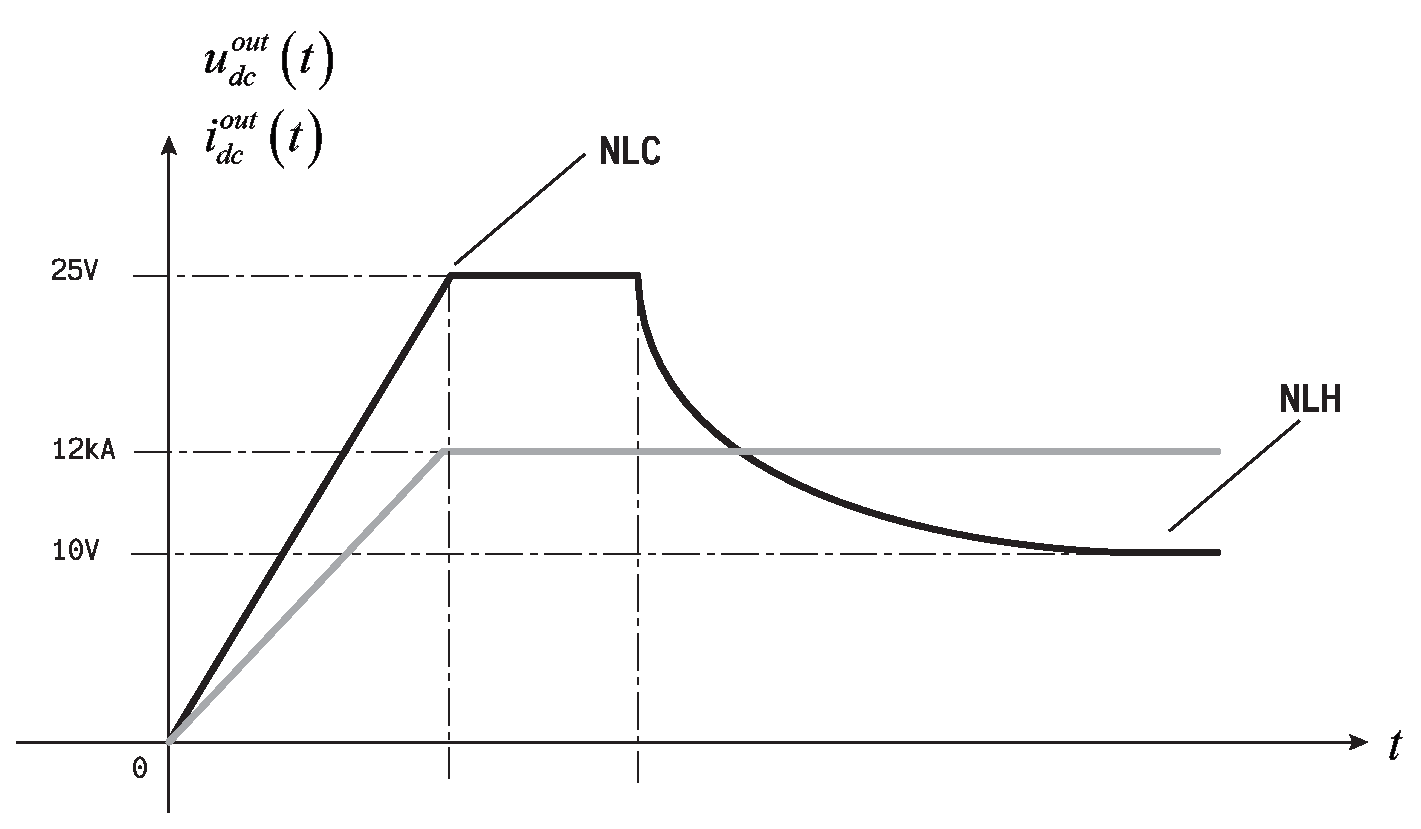
\includegraphics[width = 375pt, 
	keepaspectratio]{figures/current_profile.eps}
	\captionsetup{width=.75\textwidth}
	\caption{Load current and voltage profile under different operative conditions (NLC and NLH).}
	\label{current_profile} 
\end{figure}

\section{Power Supply Architecture}\label{sec:design}
The demanding nature of this specification — in particular the combination of very high
output current, tight ripple and regulation requirements, and the need for galvanic
isolation — calls for a carefully selected power conversion architecture. The proposed solution (as suggested by SERCOM srl) consists of two power conversion stages:
\begin{itemize}
	\item[--] an Active Front End (AFE) rectifier;
	\item[--] an isolated DC/DC converter based on a Full Bridge Converter (here called PS-FBC, where PS stays for phase shifted).
\end{itemize}
As shown in the power supply requirements the need to satisfy the condition of:
\begin{itemize}
	\item[--] \(\mathrm{PF} > 0.95\);
	\item[--] \(\mathrm{THD}_i < 5\%\);
	\item[--] provides the galvanic isolation.
\end{itemize}
brings to the above described solution composed bt an AFE stage (see Figure~\ref{fig:afe}) and by an PS-FBC stage (see Figure~\ref{fig:psfbc}).

\begin{figure}[H]
	\centering
	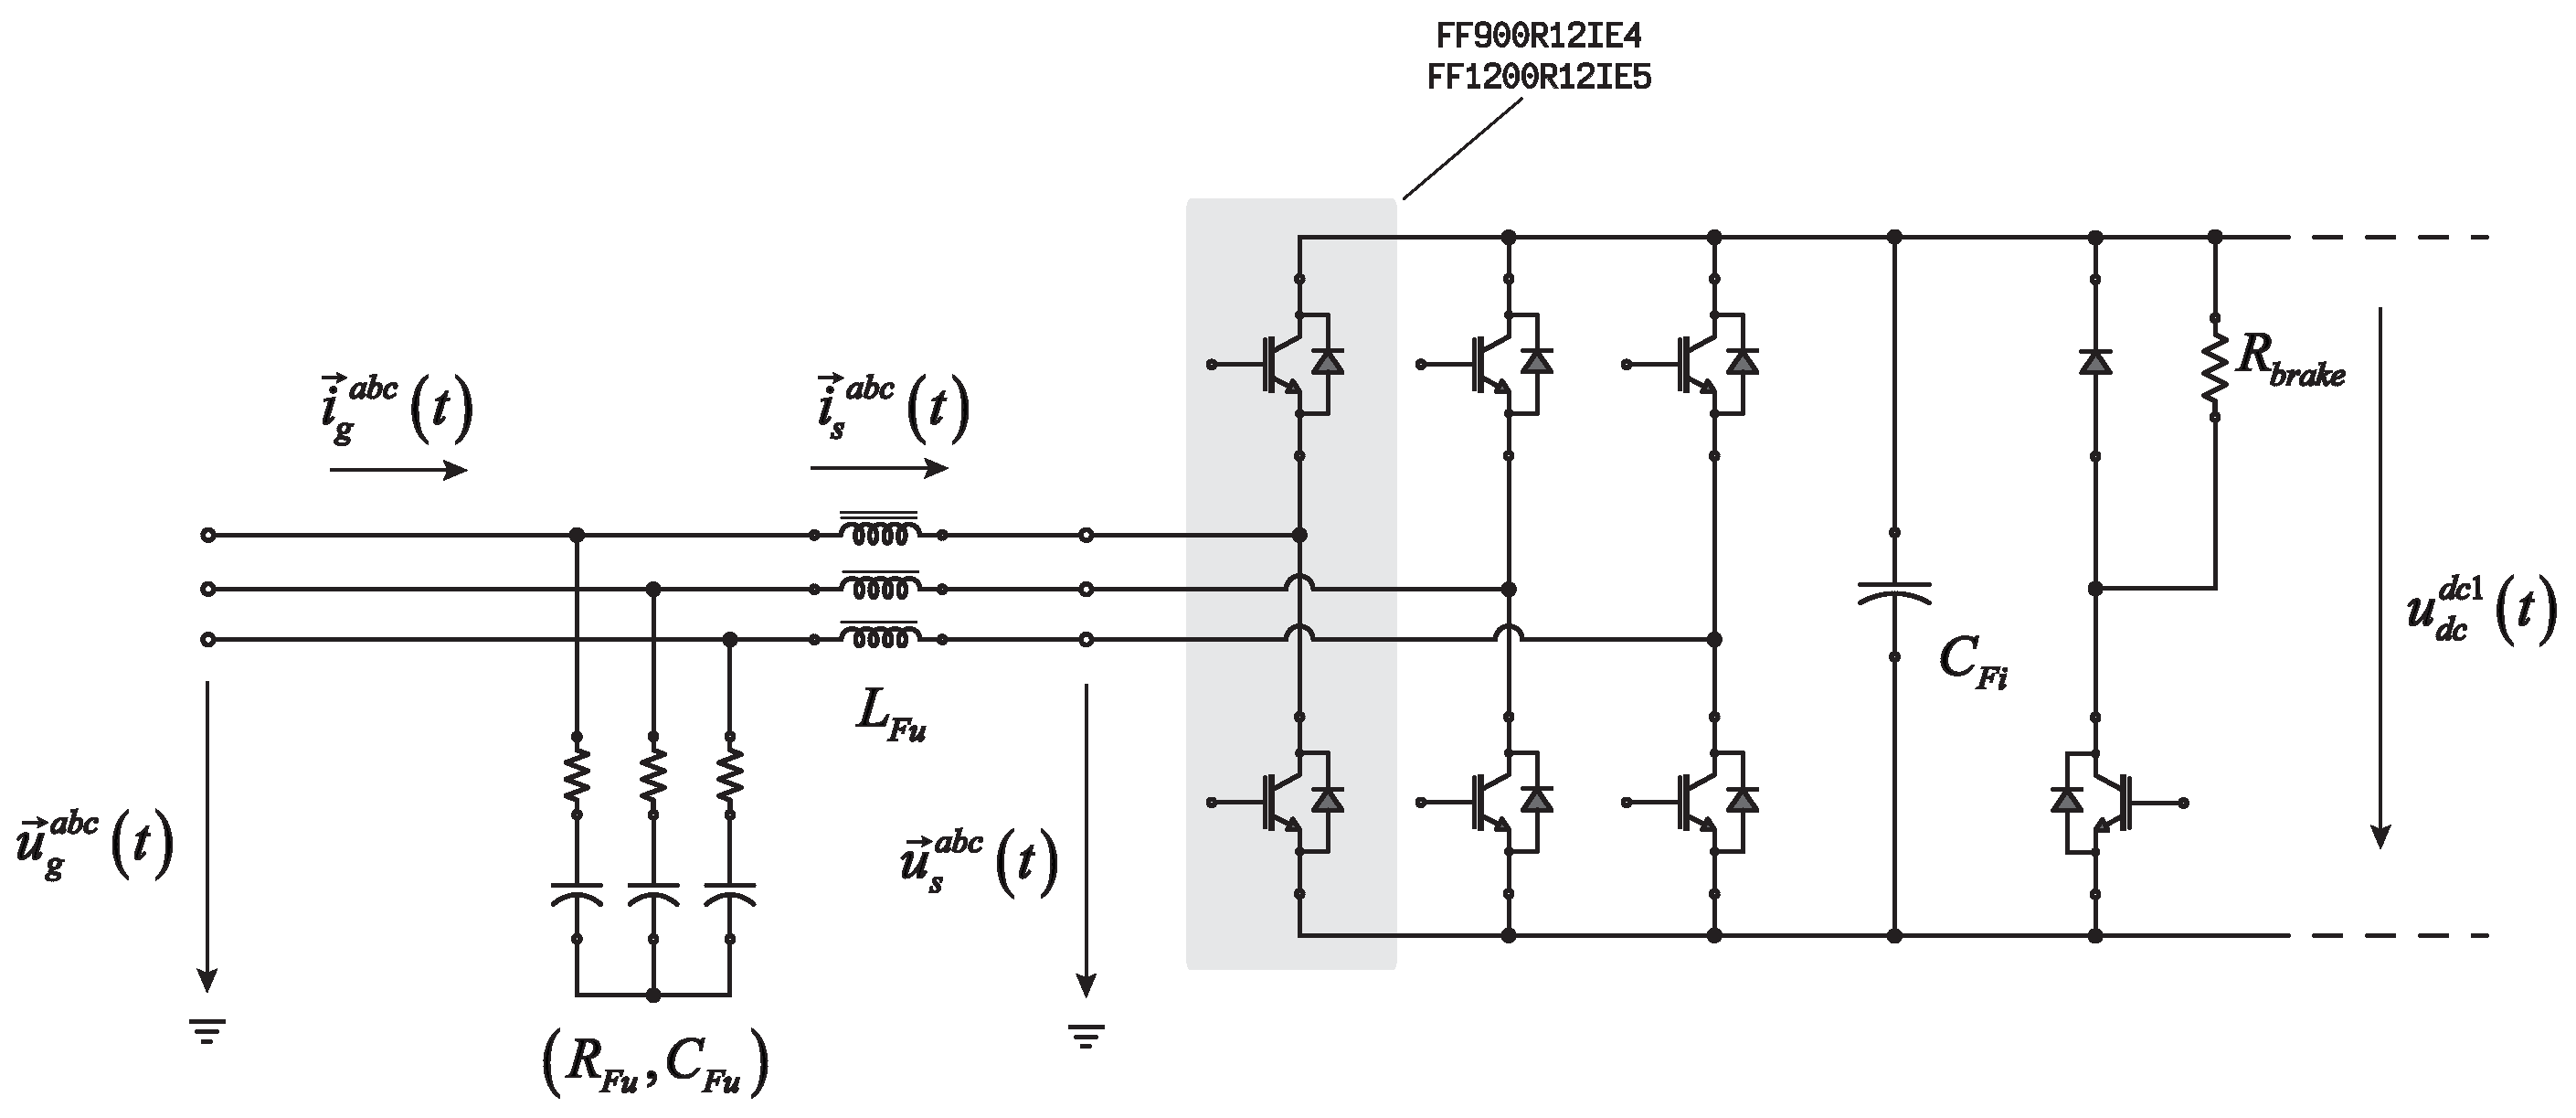
\includegraphics[width = 525pt, 
	keepaspectratio]{figures/arc/afe.eps}
	\captionsetup{width=.75\textwidth}
	\caption{Active Front End stage with LC filter layout.}
	\label{fig:afe} 
\end{figure}

\begin{figure}[H]
	\centering
	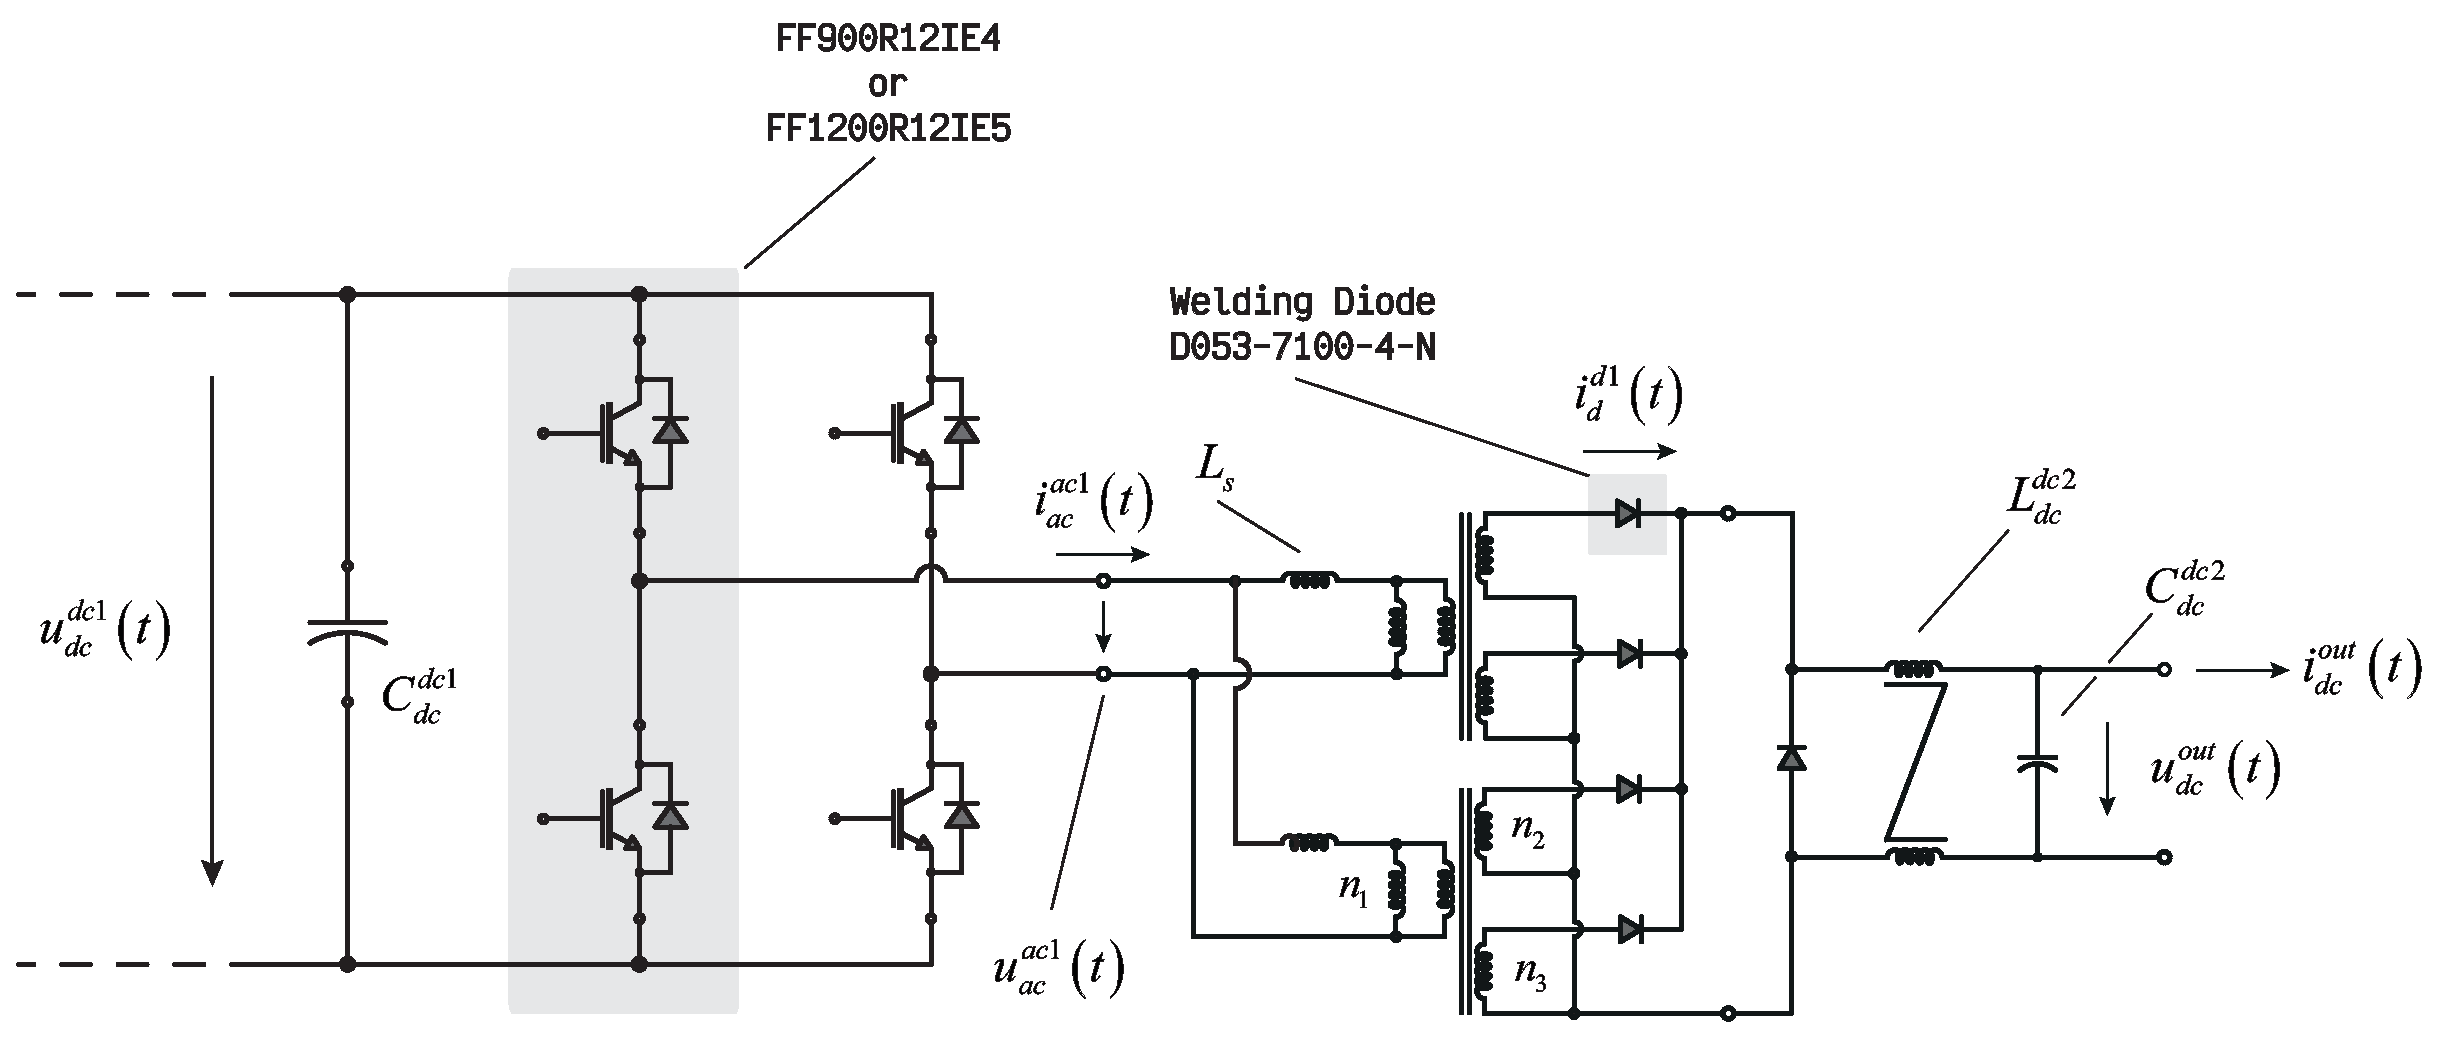
\includegraphics[width = 475pt, 
	keepaspectratio]{figures/arc/phase_shifted_full_bridge_converter_1.eps}
	\captionsetup{width=.75\textwidth}
	\caption{Full Bridge Converter layout.}
	\label{fig:psfbc} 
\end{figure}
The source inductance $L_\text{grid}$, determined by the grid short-circuit capacity
at the point of common coupling (\SI{15}{\kilo\ampere}), represents the
dominant upstream impedance seen by the AFE stage.
\begin{figure}[H]
	\centering
	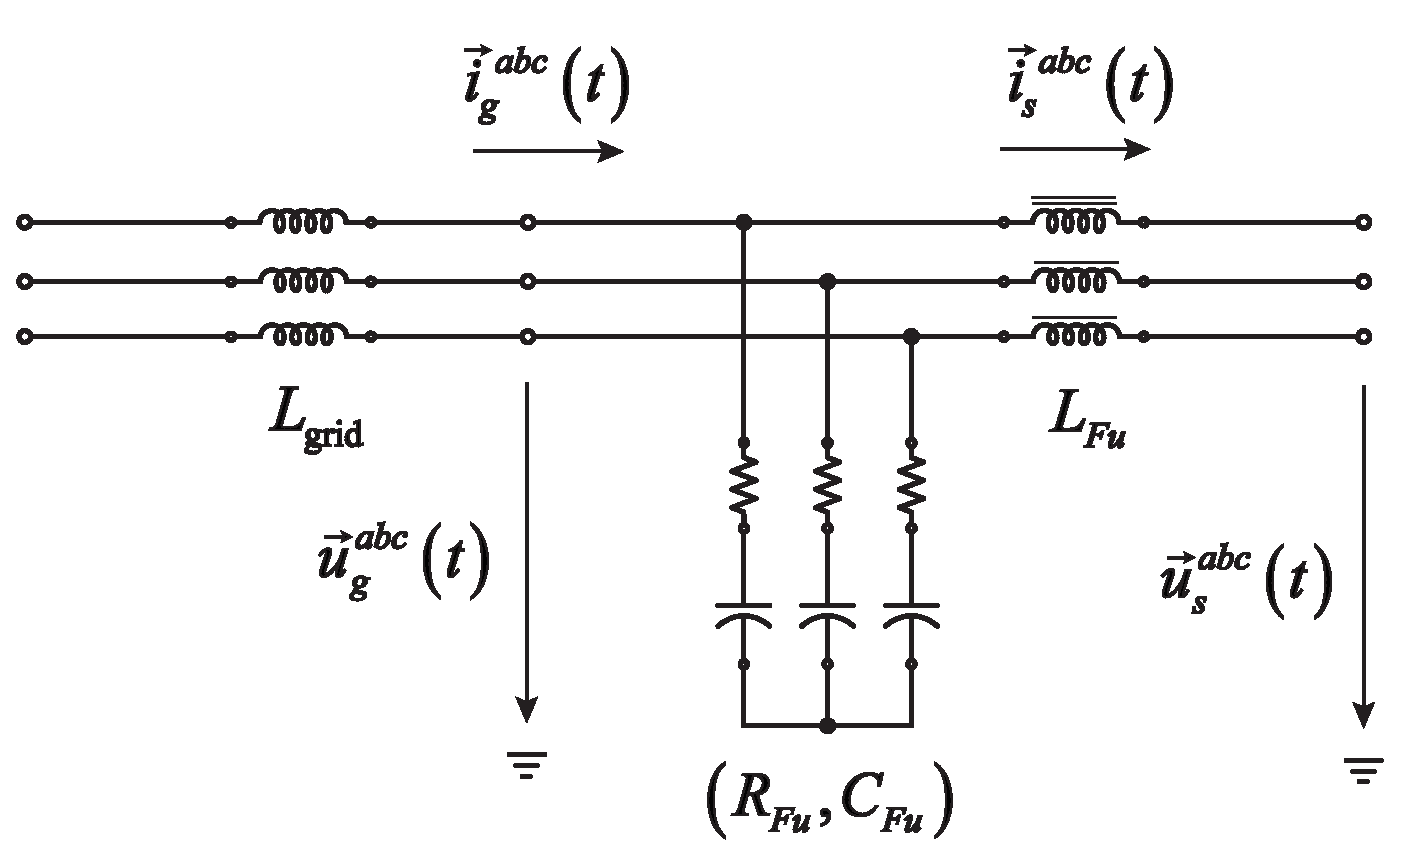
\includegraphics[width = 275pt, 
	keepaspectratio]{figures/arc/afe_grid_filter.eps}
	\captionsetup{width=.75\textwidth}
	\caption{LCL filter built using the point of common coupling (PCC) inductance.}
	\label{fig:afe_grid_filter} 
\end{figure}
\begin{figure}[H]
	\centering
	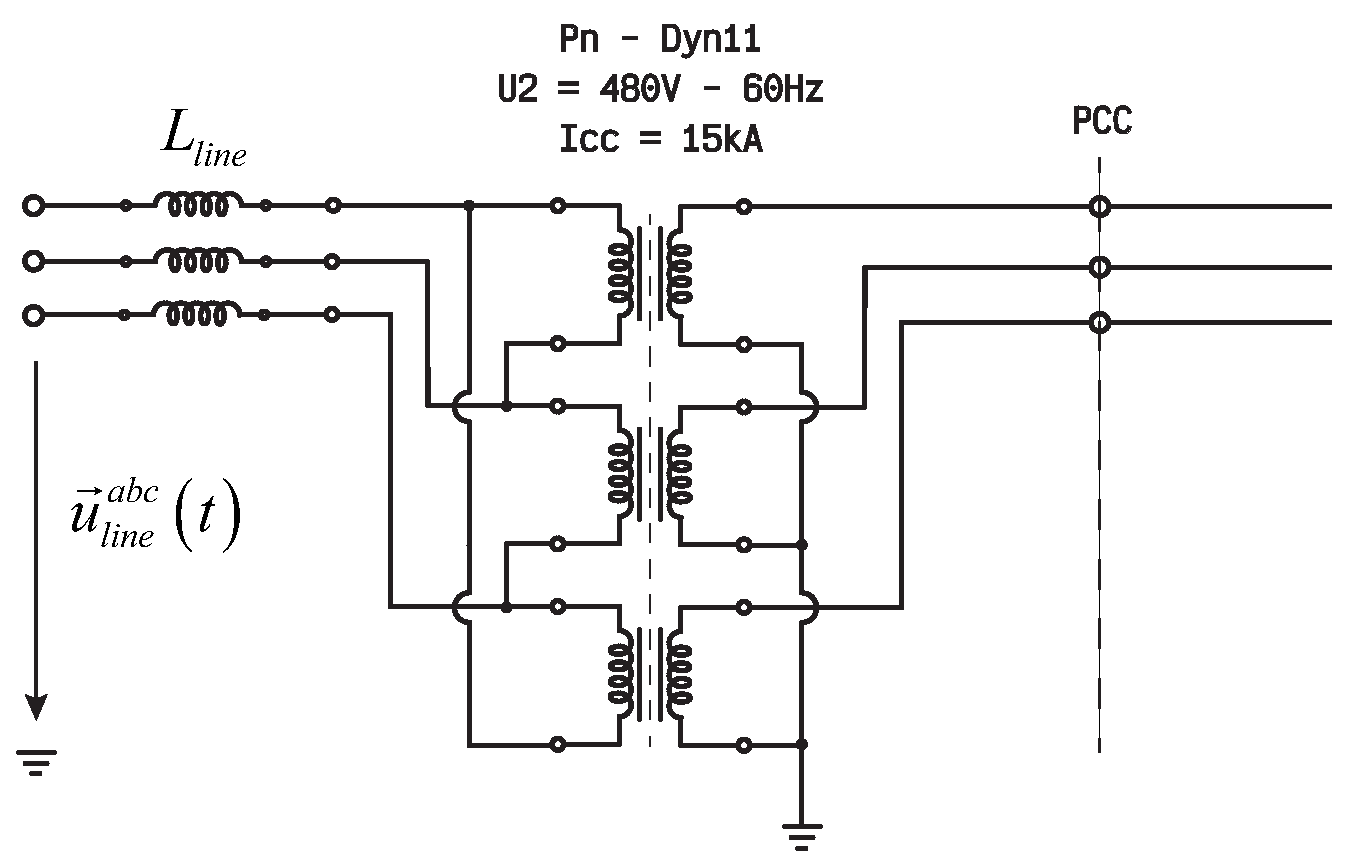
\includegraphics[width = 275pt, 
	keepaspectratio]{figures/arc/input_line.eps}
	\captionsetup{width=.75\textwidth}
	\caption{Line representation.}
	\label{fig:line_representation} 
\end{figure}

\section{Power Supply Design}\label{sec:topology}

\subsection{General design aspects}
Here a list of preliminary assumptions, and design choices:
\begin{itemize}
	\item[--] Nominal AFE power rate has been selected at $P_\text{nom}^\text{afe} = \SI{325}{\kilo\watt}$.
	\item[--] Nominal AFE stack current has been selected at $I_\text{nom}^\text{afe} = \SI{435}{\ampere}$ (rms).
	\item[--] AFE pwm switching frequency has been selected at $f_\text{pwm}^\text{afe} = \SI{4}{\kilo\hertz}$.
	\item[--] PS-FBC pwm switching frequency has been selected at $f_\text{pwm}^\text{fbc} = \SI{4}{\kilo\hertz}$ (operative frequency of the transformers).
	\item[--] The overall architecture, AFE+PS-FBC has been simulated assuming \textbf{FF900R12IE4} ($T_j^\text{max} = \SI{150}{\celsius}$) as switching device. Maximum power loss for each \textbf{module} remains below than \SI{1.4}{\kilo\watt} along the worst operative condition. Additional margin cab be achieved with \textbf{FF1200R12IE5} where $T_j^\text{max} = \SI{175}{\celsius}$.
\end{itemize}

\noindent\textbf{Remark} - the secondary rectifier stage of the PS-FBC has been implemented using
slow-recovery diodes; the Simscape model has been updated accordingly to
include a full diode model.

The selected switching frequency of \SI{4}{\kilo\hertz} represents a
design compromise. A ferrite-core transformer at this frequency results
in an excessively large and heavy magnetic component, whereas an
amorphous-iron core, while better suited to lower frequencies, introduces
significant acoustic noise at and around the switching frequency.

An improved solution — not evaluated in the present work — would consist
of replacing the slow-recovery diodes with fast-recovery rectifiers,
adopting SiC MOSFETs on the primary side, and increasing the switching
frequency to \SI{10}{\kilo\hertz}. This would allow the use of a
compact ferrite-core transformer while maintaining acceptable switching
losses.

\subsection{AFE-LCL filter topology}

\subsection{Phase Shift Full bridge Converter topology}
The series inductance $L_s$, comprising the transformer leakage inductance
$L_{lk}$ and an optional external inductor $L_{ext}$, plays a central role
in the operation of the Phase Shift Full Bridge Converter (PS-FBC) converter.
It stores the energy required to charge and discharge the IGBT output
capacitance $C_{oss}$ during the dead-time interval, thereby enabling
Zero-Voltage Switching (ZVS).
Furthermore, $L_r$ governs the power transferred between primary and
secondary according to the phase-shift angle $\varphi(t)$, and provides
inherent $\mathrm{d}i/\mathrm{d}t$ limiting during fault conditions.


%\begin{thebibliography}{99}
%	% power electronics
%	\bibitem{liserre} 
%	R. Teodorescu, M. Liserre, P. Rodrıguez, \emph{Grid converters for photovoltaic and wind power systems}. Wiley, 2011.
%\end{thebibliography}

\end{onehalfspace}
\end{document} 